\documentclass[14pt, fleqn, xcolor={dvipsnames, table}]{beamer}
\usepackage[T2A]{fontenc}
\usepackage[utf8]{inputenc}
\usepackage[english,russian]{babel}
\usepackage{amssymb,amsfonts,amsmath,mathtext}
\usepackage{cite,enumerate,float,indentfirst}
\usepackage{cancel}
\usepackage{color}
\usepackage{hyperref}
\hypersetup{colorlinks,urlcolor=NavyBlue}

\usepackage{tikz}                   
\usetikzlibrary{shadows}

% \usepackage{enumitem}
% \setitemize{label=\usebeamerfont*{itemize item}%
%   \usebeamercolor[fg]{itemize item}
%   \usebeamertemplate{itemize item}}

\graphicspath{{images/}}

\usetheme{Madrid}
\usecolortheme{seahorse}
\renewcommand{\CancelColor}{\color{red}}

\setbeamercolor{footline}{fg=Blue!50}
\setbeamertemplate{footline}{
  \leavevmode%
  \hbox{%
  \begin{beamercolorbox}[wd=.333333\paperwidth,ht=2.25ex,dp=1ex,center]{}%
    Амосов Федор, СПбГУ
  \end{beamercolorbox}%
  \begin{beamercolorbox}[wd=.333333\paperwidth,ht=2.25ex,dp=1ex,center]{}%
    Санкт-Петербург, 2014
  \end{beamercolorbox}%
  \begin{beamercolorbox}[wd=.333333\paperwidth,ht=2.25ex,dp=1ex,right]{}%
  Стр. \insertframenumber{} из \inserttotalframenumber \hspace*{2ex}
  \end{beamercolorbox}}%
  \vskip0pt%
}
\newcommand\indentdisplays[1]{%
     \everydisplay{\addtolength\displayindent{#1}%
     \addtolength\displaywidth{-#1}}}
\newcommand{\itemi}{\item[\checkmark]}

\title{Автоматическое проектирование кварталов}
\author[]{
    \small{
        Амосов Федор, СПбГУ\\
        Краевский Михаил, СПбГАСУ
    }
}
\date{}

\begin{document}

    \begin{frame}
        \maketitle
        \small
    \end{frame}

    \section{Постановка задачи}  
    
        \begin{frame}{Постановка задачи}
            2 картинки
            \begin{itemize}
                \item пустой участок
                \item застроенный участок
            \end{itemize}        
        \end{frame}
        
        \begin{frame}{Проблематика}
            10 ограничений     
        \end{frame}
        
        \begin{frame}{Проблематика}
            Картинка с задротским четежом   
        \end{frame}
        
        \begin{frame}{Машинное обучение}
            Фичи
            \begin{enumerate}
               \item Площадь участка
               \item Максимальная разрешенная высота зданий на участке
               \item Периметр участка
            \end{enumerate}
            Ответы
            \begin{enumerate}
               \item Жилая площадь
               \item Школы
               \item Садики
               \item Парковки
               \item ...
            \end{enumerate}           
        \end{frame}
        
        \begin{frame}{Майнинг данных}
            Упоротые картинки mapinfo (РГИС)    
        \end{frame}
        
        \begin{frame}{Майнинг данных}
            Картинка с 48 этажным домом
        \end{frame}
        
        \begin{frame}{Модели для обучения}
            Данные по разным моделькам
        \end{frame}
        
        \begin{frame}{Похожие проекты}
            Картинка в трехмерье
        \end{frame}
        
        \begin{frame}{Архитектура проекта}
            \begin{center}
                \includegraphics[scale=0.25]{architecture.jpg}
            \end{center}
        \end{frame}
        
        \begin{frame}{Хостинг}
            \begin{center}
                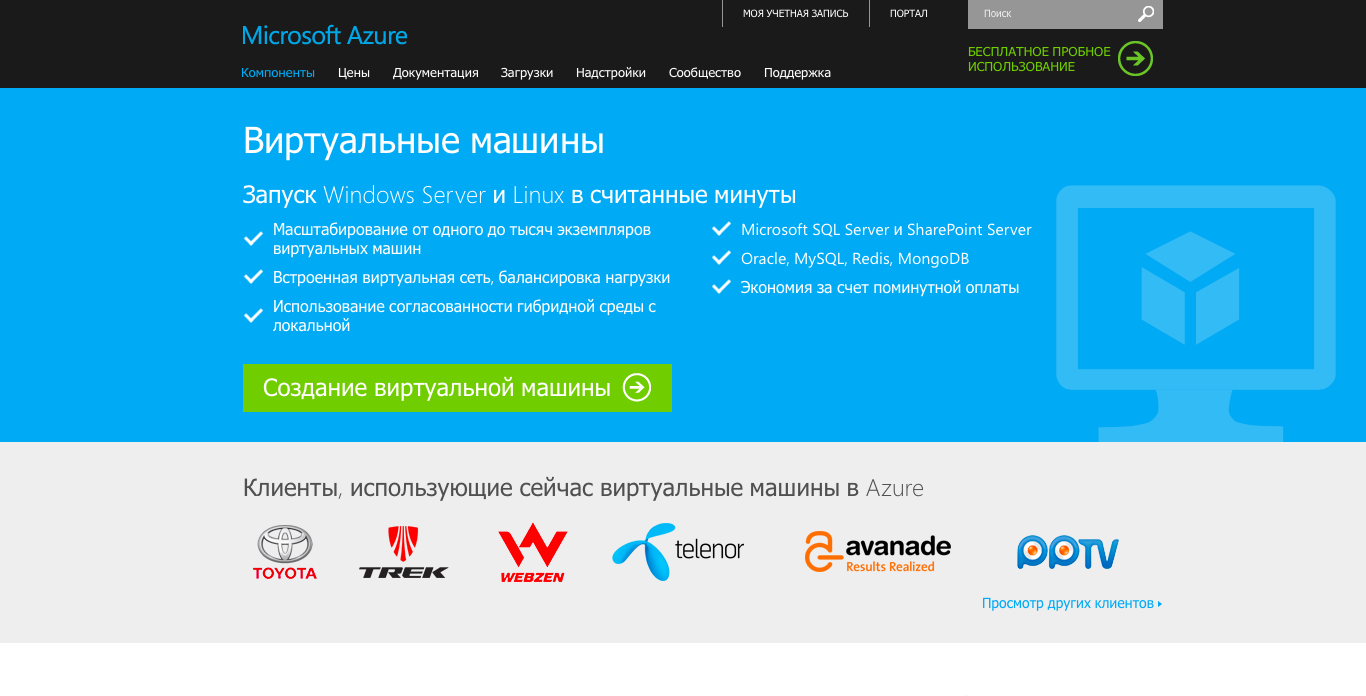
\includegraphics[scale=0.25]{azure.png}
            \end{center}
        \end{frame}
        
        \begin{frame}{В итоге}
            \begin{center}
                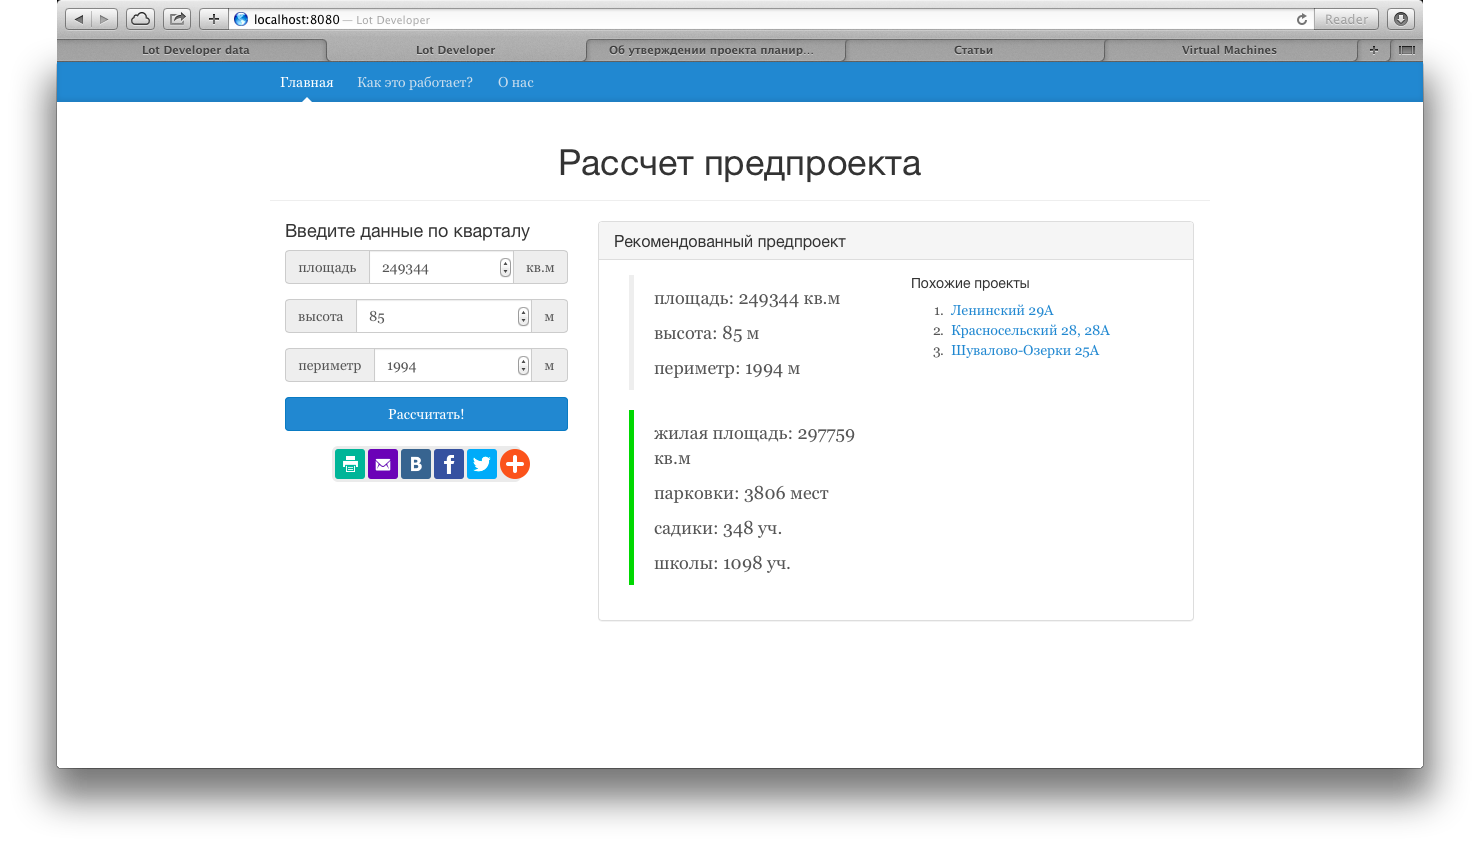
\includegraphics[scale=0.23]{example.png}
            \end{center}
        \end{frame}
        
        \begin{frame}{Используемые технологии}
            \begin{description}
                \item [Сервер]
                    \begin{itemize}
                        \item Java + Spring Framework + Jetty
                        \item Maven
                        \item Spring MVC + JSP
                        \item \bf{Goole Docs API}
                    \end{itemize}
                ~\\
                \item [Клиент]
                    \begin{itemize}
                        \item HTML + CSS + Bootstrap
                        \item JavaScript + jQuery + Ajax
                    \end{itemize}
                ~\\
                \item [Система контроля версий]
                    \begin{itemize}
                        \item Git
                    \end{itemize}
            \end{description}
        \end{frame}
        
        \begin{frame}{Q\&A}
            \begin{center}
                Спасибо за внимание!\\
                \href{http://ciblock.cloudapp.net}{ciblock.cloudapp.net}
            \end{center}
        \end{frame}


\end{document}